\documentclass[12pt]{article}
\usepackage{../eplcrypto}
\usepackage{geometry} % see geometry.pdf on how to lay out the page. There's lots.
\geometry{a4paper} % or letter or a5paper or ... etc
% \geometry{landscape} % rotated page geometry
\usepackage[parfill]{parskip}
% See the ``Article customise'' template for come common customisations
\usepackage{amsmath}
\usepackage{graphicx}
\usepackage{amssymb}
\usepackage{algorithmic}
\usepackage{algorithm}
\title{Slides03}

%%% BEGIN DOCUMENT
\begin{document}


\maketitle
\tableofcontents
\newpage
\section{Reminder}
\subsection{ Experiment $\PrivKeav$}
\textbf{Experiment} $\PrivKeav(n)$
\begin{enumerate}
\item $\mathcal{A}(1^n)$ outputs $m_0,m_1$ of identical lengths
\item pick $k \leftarrow Gen(1^n)$ and  $b \leftarrow \{0,1\}$ and send $c \leftarrow Enc_k(m_b)$ to $\mathcal{A}$
 \item $\mathcal{A}(c)$ outputs $b'$
 \item Define $Priv_{\mathcal{A},\prod}^{eav}(n):=1$ iff $b=b'$
\end{enumerate}
$\Pi \define \langle \Gen, \Enc, \Dec \rangle $ has \emph{indistinguishable} encryptions in the presence of eavesdroppers if $\forall$ PPT $\mathcal{A}$, $\exists$ negl. $\epsilon$:
\begin{equation*}
Pr[\PrivKeav(n)] = \frac{1}{2} + \epsilon(n)
\end{equation*}

\section{Building Encryption Schemes}
So far we have seen encryption schemes for one single message, how do these schemes extend to several messages? We also have seen that using the same key to encrypt more than one message made one-time pad insecure. It is possible to use different key for each message but then the question of how it is transferred and how efficient it is comes into play. As a first step, the definition of security is needed for multiple messages.\\
\subsection{Secure multiple encryption}
%EXPERIMENT MULT
Define the multiple-message eavesdropping experiment $\PrivKmult$(n)

\begin{enumerate}
\item $\A$ outputs $M_0 = (m_0^1,\dots,m_0^t)$, $M_1 = (m_1^1,\dots,m_1^t)$
\item Choose $k \leftarrow Gen(1^n)$ and $b \leftarrow \{0,1\}$, and send ($Enc_k(m_b^1),\dots,Enc_k(m_b^t)$) to $\A$
\item $\A$ outputs $b'$
\item Define $\PrivKmult$(n)$\define 1$ iff $b=b'$
\end{enumerate}
\newpage
$\Pi \define \langle \Gen, \Enc, \Dec \rangle$ has \emph{indistinguishable multiple encryption} in the presence of eavesdroppers if\\
$\forall$ PPT $\A$, $\exists \negl$:
\begin{equation*}
Pr[\PrivKmult(n)] = \frac{1}{2} + \epsilon(n)
\end{equation*}
\textbf{Without maintaining a state between encryptions, we cannot achieve acceptable security with a deterministic scheme.}\\\\
\textbf{Probabilistic encryption:}
\begin{itemize}
\item The same message, encrypted with the same key, yields different results
\item The decryption remains deterministic.
\end{itemize}
\subsection{Security against Chosen-Plaintext Attacks (CPA)}
So far in the course, the adversaries have been passive. What they did was to eavesdrop on ciphertext, and tried to recover some information on the ciphertext.\\
But a real-world adversary could have access to additional information.
\begin{itemize}
\item Previous encryptions (with same key) of messages he knows
\item Previous encryptions (with same key) of messages he has chosen
\item ...
\end{itemize}

\subsubsection{New adversary}
\begin{itemize}
\item Access to an encryption oracle $\Enc_k(\cdot)$ that will encrypt messages of his choice.
\item Allowed to call oracle adaptively, before and after submitting two challenge messages $m_0, m_1$ of his choice
\item As before, must tell his bit $b'$ choice
\end{itemize}

\subsection{ Experiment $\PrivKcpa$}
\textbf{Experiment} $\PrivKcpa(n)$
\begin{enumerate}
\item Pick $k \leftarrow Gen(1^n)$ 

\item $\A$ is given oracle access to $\Enc_k(\cdot)$

\item $\A(1^n)$ outputs $m_0,m_1 \in \M$

\item Choose $b \leftarrow \{0,1\}$ and send $c = \Enc_k(m_b)$ to $\A$

\item $\A$ is again given oracle access to $\Enc_k(\cdot)$

 \item $\A(c)$ outputs $b'$

 \item Define $\PrivKcpa(n):=1$ iff $b=b'$

\end{enumerate}
$\Pi \define \langle \Gen, \Enc, \Dec \rangle $ has \emph{indistinguishable} encryption under a chosen-plaintext attack if $\forall$ PPT $\A$, $\exists$ negl. $\negl$:
\begin{equation*}
Pr[\PrivKcpa(n)] = \frac{1}{2} + \negl(n)
\end{equation*}
\textbf{CPA-security implies security against an eavesdropper.}\\\\
Why not we ask in 5th step of the $\PrivKcpa$ that $\A$ cannot ask for encryption of $m_0$ or $m_1$? Well, when we have a probabilistic encryption scheme which means even if $\A$ asks this, it will not give too much information to him in the experiment.\\\\

\subsubsection{Extending the CPA-security definition and relations}
\begin{itemize}
\item CPA-security for single encryption $\rightarrow$ CPA-security for multiple encryption
\end{itemize}

\textbf{CPA $\rightarrow$ Multiple message eavesdropper $\rightarrow$ Eavesdropper}

\subsection{Constructing CPA-secure encryption scheme}
Idea for a probabilistic encryption scheme:\\
Change $\Enc$ as follows:
\begin{itemize}
\item Pick $r \leftarrow \{0,1\}^n$ and encrypt $m$ as $\langle r, G(k||r)\oplus m \rangle$
\end{itemize}
$G$, as the PRG, is only guaranteed to output pseudorandom values with a secret seed.\\
Therefore, there is a need for something stronger than a PRG. A function F  that when $r$ is public (but not k),  F(k,r) is pseudorandom.

\subsubsection{Pseudorandom Functions}
Pseudorandom functions generalize the concept of pseudorandom generators. Rather than focusing on strings that look random, we are now interested in functions that exhibit a "random-like" behavior. Now, when we talk about pseudorandomness, it doesn't make much sense to say that a specific, fixed function $f: \{0,1\}^* \rightarrow \{0,1\}^*$ is pseudorandom. This is similar to saying that any fixed function is random, which doesn't have a meaningful interpretation. Instead, we need to consider the pseudorandomness of a distribution of functions. This distribution arises when we think about keyed functions.

A keyed function $F: \{0,1\}^* \times \{0,1\}^* \rightarrow \{0,1\}^*$ is a two input function, where the first input is called the \emph{key} and denoted by $k$. The security parameter $n$ indicates the key length, input length, and output length. \\

Let $\textbf{Func}_n$ denote the set of all functions mapping $n$-bit strings to $n$-bit strings.
In typical usage a key $k \in \{0,1\}^n$ is chosen and fixed, and we are then interested in single-input function $F_k:  \{0,1\}^n \rightarrow \{0,1\}^n$ defined by $F_k(x) \define F(k,x)$ mapping $n$-bit input strings to $n$-bit output strings.\\

Keyed function $F$ and distribution of functions:
\begin{itemize}
\item A keyed function $F$ creates a distribution of functions in $\textbf{Func}_n$
\item This distribution is formed by choosing a random key $k \in \{0,1\}^n$ and then considering the resulting single-input function $F_k$
\end{itemize}

Pseudorandomness of $F$:
\begin{itemize}
\item $F$ is called pseudorandom if, when we apply it with a uniformly chosen key $k$ to create $F_k$, the resulting function $F_k$ is indistinguishable from a function chosen uniformly at random from the set of $\textbf{Func}_n$.
\end{itemize}

\newpage
\emph{Let $\textbf{Func}_n$ denote the set of all functions mapping $n$-bit strings to $n$-bit strings.}\\ 
How many functions there are in $\textbf{Func}_n$?
\begin{itemize}
\item What is a function in our case?\\
One-to-one correspondence from domain $D = \forall x \in \{0,1\}^n$ to range  $R = \forall x \in \{0,1\}^n$ (they are the same in our case).
\item How many functions there are mapping n-bit strings to n-bit strings?\\
Think about a look up table as below:
\begin{table}[h]
  \centering
  \begin{tabular}{|c|c|}
    \hline
    $x$ & $f(x)$ \\
    \hline
    1 & $a$ \\
    2 & $b$ \\
    3 & $c$ \\
    \hline
  \end{tabular}
  \caption{Example lookup table.}
  \label{tab:your_table_label}
\end{table}
x is mapped to f(x), in our case the domain and range are n-bits, which means there are $2^n$ entries in the table (values that cover the n-bit input x). Also, the output of the function, $(x)$ is n bits, so this means that $a$ in the example above is an n-bit number. \\
So, a function in  $\textbf{Func}_n$ can be described by $2^n\times n$ bits ($2^n$ entries where each entry is n-bits). Think about this as a one huge number of $2^n\times n$-bits, how many different values can this $2^n\times n$-bit number can have $\rightarrow$ $2^{2^n\times n}$. Therefore, there are $2^{2^n\times n}$ functions in $\textbf{Func}_n$.
\item What does it mean to select a uniform function $f \in \textbf{Func}_n$?\\
It means to select each row in the lookup of $f$ table uniformly.
\end{itemize}

\textbf{What is now a pseudorandom function?}
\begin{itemize}
\item It is a keyed function $F$ such that $F_k$ (for uniform $k\in \{0,1\}^n$) is indistinguishable from $f$ for uniform  $f \in \textbf{Func}_n$. The PRF is chosen from a distribution over (at most) $2^n$ distinct functions, whereas $f$ is chosen from all $2^{2^n\times n}$ in $\textbf{Func}_n$
\end{itemize}
The set of functions \( F \) can take on is limited to \( 2^n \) distinct possibilities, making it a smaller, more manageable set compared to the vast set of all possible functions. The pseudorandomness property ensures that, to an observer, the behavior of \( F_k \) with a chosen key is as good as interacting with a function randomly selected from the smaller set \( \textbf{Func}_n \).
\subsubsection{Indistinguishability}
$F: \{0,1\}^* \times \{0,1\}^* \rightarrow \{0,1\}^*$ is a pseudorandom function if $\forall$ PPT $D$, $\exists$ negl. $\negl$:
\begin{equation*}
|Pr[D^{F_k(\cdot)}=1]-Pr[D^{f(\cdot)}=1]| \le \negl(n)
\end{equation*}
\begin{itemize}
\item k is chosen uniformly at random in $\{0,1\}^n$
\item D is not given the key k
\item As D is PPT, he can only do a polynomially bounded number of oracle queries.
\end{itemize}
\textbf{Pseudorandom functions exit iff pseudorandom generators exit.}

\subsubsection{Building a CPA-secure scheme from a PRF}
Define $\Pi \define \langle \Gen, \Enc, \Dec \rangle$ as:\begin{itemize}
\item $\Gen:$ Choose random $k\leftarrow \{0,1\}^n$
\item $\Enc:$ on input $m,k \in  \{0,1\}^n$
	\begin{itemize}
	\item Choose random $r\leftarrow \{0,1\}^n$
	\item $c\define \langle r,F_k(r)\oplus m\rangle$
	\end{itemize}
\item $\Dec:$ on input $k \in\{0,1\}^n$ and $c = \langle r,s \rangle$ output $m\define s\oplus F_k(r)$
\end{itemize}
\textbf{Theorem:} If $F$ is a pseudorandom function, this construction has indistinguishable encryption under a chosen-plaintext attack.\\

\subsection{Proof for CPA-secure scheme from a PRF}
In two steps.
\begin{itemize}
\item Prove that the scheme is secure if $F_k$ is replaced by a truly random function.
\item Prove that if the scheme (with $F_k$) were insecure, we could distinguish $F_k$ from a truly random function.
\end{itemize}

\subsubsection{Step 1: Idealized scheme}
Replacing $F_k$ with a truly random function $f$. Consider a CPA-adversary $\A$:
\begin{itemize}
\item Uses oracle $\O$ to encrypt messages of his choice.
\item Outputs $m_0,m_1$
\item Receives $c = \langle r,f(r)\oplus m_b \rangle$ with random $b \in \{0,1\}$
\item Uses oracle $\O$ to encrypt messages of his choice
\item Outputs $b'$
\end{itemize}
Note: $\A$ makes at most. $q(n)$ oracle queries in total, what are his changes of success?\\
\textbf{Two cases:}
\begin{enumerate}
\item r is never used by oracle except for $m_b$  
\begin{itemize}
\item Then $\A$ learns nothing useful from oracle queries. $==>$ $\A$'s chance of success is $1/2$, same as one-time pad.
\end{itemize}

\item r has been used at least once by oracle
\begin{itemize}
\item $\A$ has $\langle r,f(r)\oplus m_b \rangle$ and $\langle r,f(r)\oplus m' \rangle$ for some $m'$ he knows
\item $\A$ can easily deduce $f(r)$ and hence the value of $b$.
\item $\A$ always wins in this case\\\\
Note: Probability for this case to happen is $\frac{q(n)}{2^n}$
\end{itemize}
\begin{align*}
\Pr[\PrivKcpa(n)=1] &= \Pr[\PrivKcpa(n)=1 \, \land \, \text{Repeat}] + \Pr[\PrivKcpa(n)=1 \, \land \, \overline{\text{Repeat}}] \\
&\le \Pr[\text{Repeat}] + \Pr[\PrivKcpa(n)=1 \, | \, \overline{\text{Repeat}}]\\
&\le \frac{q(n)}{2^n} + \frac12
\end{align*}
When repeat happens you always win, when it does not happen, you have the best chance of $\frac12$. So probability of repeat times 1 (since you always win) plus the probability of winning given that repeat does not happen.
\end{enumerate}

\subsubsection{Step 2: Real scheme is as good as idealized one}
Suppose that there exits $\A$ that can break the (real, the one with $F_k$) scheme with non-negligible probability $\frac12 + \eta(n)$
\newpage
\textbf{Reduction:}
\begin{figure}[ht]
    \centering
    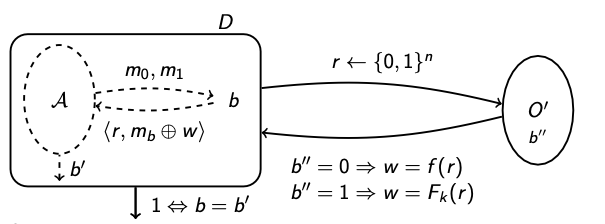
\includegraphics[width=12cm]{figures/f1.png}
    \caption{Reduction}
\end{figure}

So:
\begin{itemize}
\item If $b''=0$ $Pr[D=1] \le \frac12 + \frac{q(n)}{2^n}$ : idealized scheme
\item If $b''=1$ $Pr[D=1] = \frac12 + \eta(n)$ : normal security game 
\item $D$ distinguishes with Pr $\ge \eta(n)-\frac{q(n)}{2^n}$
\end{itemize}
\begin{equation*}
|Pr[D^{F_k(\cdot)}(1^n)=1]-Pr[D^{f(\cdot)}(1^n)=1]| \ge \eta(n)-\frac{q(n)}{2^n}
\end{equation*}
Since, $F$ is a PRF, $\eta(n)-\frac{q(n)}{2^n}$ must be negligible, so $\eta(n)$ must be negligible.

Small summary:
\begin{itemize}
\item If we use a truly random function in the construction, then the scheme is secure
\item If someone can break the scheme with a practical function $F_k$, then he can distinguish $F_k$ from a truly random function.
\end{itemize}
\emph{If $F_k$ is a PRF, the scheme is secure.}
\subsection{Multiple message security}
CPA-security implies multiple-message security, but focuses on the confidentiality of one message.
\begin{itemize}
\item When we encrypt l messages, what is the probability that we draw the same r more than once?
\item How many messages can we encrypt before being at risk?
\end{itemize}
\newpage

\subsubsection{The birthday paradox}
\emph{How many people do we need in a room to have a probability of at least one half that two of them have the same birth date?}

The birthday paradox is a famous problem in probability theory. It deals with the surprising fact that the probability of two people sharing the same birthday is higher than one might intuitively expect.

\subsubsection*{Probability Calculation}

If there are only two people in a group, the probability that they share the same birthday is $\frac{1}{365}$ (assuming a non-leap year with 365 days).

As you add more people to the group, the probability of at least two people sharing the same birthday increases.

The surprising result is that you only need around 23 people in a group for there to be a better-than-even chance (more than 50\%) that two of them share the same birthday.

\subsubsection*{Formula}

The probability can be calculated using combinatorics, but a simplified version is:
\[
P(\text{{at least one shared birthday}}) = 1 - \frac{365}{365} \times \frac{364}{365} \times \frac{363}{365} \times \ldots \times \frac{365 - n + 1}{365}
\]
where \( n \) is the number of people in the group.

More simply:\\
 If you are randomly selecting values from a space of size N, the probability of encountering a collision (i.e., selecting the same value more than once) becomes significant after about $\sqrt{N}$ selections ($\sqrt{365} \approx 19$ ).
 
 So, the risk to "draw" the same $r$ twice is driven by the birthday paradox. Negligible if the number of messages is negligible compared to $2^{n/2}$ where n is the block length.\\
 \emph{Number of blocks is polynomial, $2^{n/2}$ is exponential.}\\
 Remarks:
 \begin{itemize}
\item This means that not only key size but also the block size (data processed at a time) is a security factor. (DES had blocks of size 64 bits)
\item AES, the most widely used PRF today, has blocks of size 128 bits, independently of the key size.
\end{itemize}
\newpage
 
\section{Modes of Operation and Encryption in Practice}
\subsection{Stream Ciphers}
We cannot use a PRG $G$ with expansion factor $l$ to encrypt messages of length $l' > l$ using a single n-bit key. We can encrypt messages of length $l' < l $ by truncating the output of $G$, doing this is wasteful since it involves discarding generated values.

Here, \emph{stream ciphers} come into play. They are used in practice to instantiate PRGs, and they provide flexibility. The outputs bits of a stream cipher are produces gradually and on demand, so that an application can request exactly as many pseudorandom bits as it needs.

Formally a stream cipher is a pair of deterministic algorithms $\langle$ Init, Next $\rangle$:
\begin{itemize}
\item \textbf{Init}: Takes as input a seed s and an optional \emph{initialization vector IV}, and outputs. some initial state \textbf{st}
\item \textbf{Next:} Takes as input a current state \textbf{st} and output a bit (in practice the output might be a byte or even larger number of bits) $y$ along with updated state  \textbf{st'}
\end{itemize}

As a shorthand \textbf{GetBits} is used which takes an initial state $st_0$ and a desired output length $l$ which then returns $l$-bit string and the final state $st_0$
We let \textbf{GetBits}$_1$ be the algorithm that runs \textbf{GetBits} and only returns its initial output, the $l$-bit string.


A secure stream cipher without an $IV$ is just a PRG with a flexible interface.
Formally defined, a stream cipher $\langle$ Init, Next $\rangle$ and a parameter $l = l(n) > n $ we define the deterministic function $G^l$:
\begin{equation*}
G^l(s) \define \textbf{GetBits}_1(\text{Init(s)}),1^l)
\end{equation*}
Then the stream cipher $G^l$ is secure if it a PRG for any polynomial $l$.
Security for a stream cipher that does take an IV can be defined in multiple
ways. We define security in this case to be akin to that of a pseudorandom
function.
\begin{equation*}
F_s^l(IV) \define \textbf{GetBits}_1(\text{Init(s,IV)}),1^l)
\end{equation*}
Then the stream cipher is secure if $F^l$ is a PRF for any polynomial $l$. Practical stream ciphers typically do not support arbitrary values of n
(which determines the length of the seed and the IV), but instead work only
for some fixed values of n. Concrete-security definitions are thus more appro-
priate than the asymptotic definitions given above
\subsection{Stream-cipher modes of operation}
\subsubsection{Synchronized mode}
Stream ciphers are often used to encrypt an online communication session between two parties. A stateful communication where the sender and receiver are required to maintain state between the encryption/decryption of different messages.

Observe that for synchronized mode, the stream cipher does not need to
use an $IV$.
\subsubsection{Unsynchronized mode}
When a stream cipher does take an IV, it can be used to construct a stateless encryption scheme, the main advantage here is that the encryption scheme directly handles arbitrary-length messages.

\subsection{Block ciphers and block-cipher modes of operation}
A block cipher is simply anothe name for a (strong) pseudorandom permutation. That is, a block cipher $F: \{0,1\}^n \times \{0,1\}^l \rightarrow \{0,1\}^l$ is a keyed function such that, for all $k$, the function $F_k$ defined by $F_k(x) \define F(k,x)$ is a bijection (a permutation). Recall that $n$ is the \emph{key length} of $F$ and $l$ is its \emph{block length}.

The main distinction between block ciphers and pseudo random permutations is that the former typically only support a specific set of key/block lengths, and in particular do not support arbitrary-length keys. For simplicity, we will assume in this section that $l=n$.

\textbf{we can use any block cipher F to implement the stream-cipher modes of operation}
\begin{equation*}
m=m_1,m_2,\dots,m_l \quad \forall i \in \{1,\dots,l\}\,, m_i \in \{0,1\}^n
\end{equation*}
Messages are assumed to have lengths multiples of n, this does not sacrifice generality.
\newpage
\subsubsection{Electronic Code Book (ECB) mode}
This is a naive mode of operation in which the ciphertext is obtained by direct application of the block cipher to each plaintext block. The decryption is done by computing $F_k^{-1}$ given that it is efficiently computable. 
\begin{figure}[ht]
    \centering
    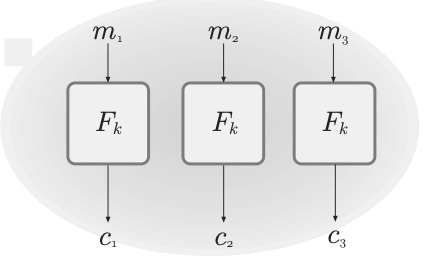
\includegraphics[width=8cm]{figures/f2.png}
    \caption{ECB mode}
\end{figure}
ECB is deterministic and therefore cannot be CPA-secure, worse it is not even EAV-secure. A repeating sequence in plaintext will result in a repeating block in the ciphertext. Thus, for example, it is easy to distinguish the encryption of a plaintext that consists of two identical blocks from the encryption of a plaintext that consists of two different blocks.
\newpage
\subsubsection{Cipher Block Chaining (CBC) mode}
To encrypt here, a uniform initialization vector (IV) of length n is first chosen as the initial ciphertext block. Then, ciphertext blocks are generated by applying the block cipher to the XOR of the current plaintext block and the previous ciphertext block.
\begin{figure}[h]
    \centering
    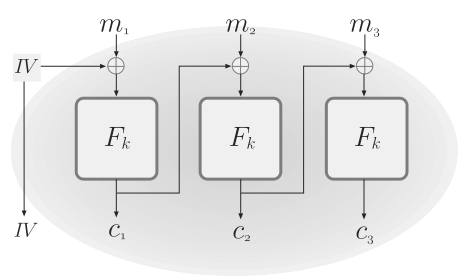
\includegraphics[width=8cm]{figures/f3.png}
    \caption{CBC mode}
\end{figure}

\textbf{Theorem:} If F is a PRP, then CBC mode is CPA-secure\\

The main drawback is that the encryption needs to be done in sequential manner, thus it cannot take advantage of parallel processing.

\subsubsection*{Chained CBC mode}
There is a stateful variant of CBC-mode encryption called "chained CBC mode" in which the last block of the previous ciphertext is used as the IV when encrypting the new message.
\begin{figure}[h]
    \centering
    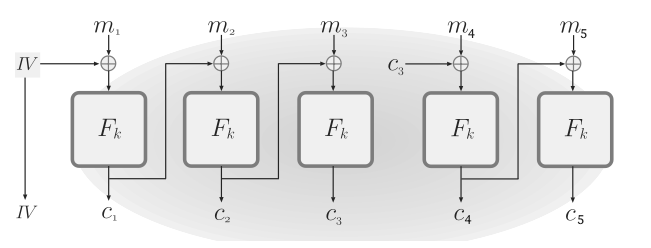
\includegraphics[width=8cm]{figures/f4.png}
    \caption{Chained CBC mode}
\end{figure}

Chained CBC mode is vulnerable to a chosen-plaintext attack. The basis of the attack is that the adversary
knows in advance the “initialization vector” $c_3$ that will be used for the second encrypted message
 \subsubsection{Counter (CTR) mode}
Counter mode can be viewed as an unsynchronized stream-cipher mode, where the stream cipher is constructed from the block cipher $F$.
 \begin{figure}[h]
    \centering
    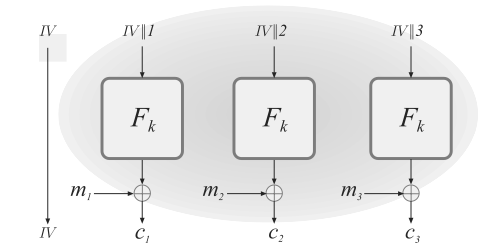
\includegraphics[width=8cm]{figures/f5.png}
    \caption{CTR mode}
\end{figure}

To encrypt a message with $l < 2^{n/4}$ blocks using CTR mode, a uniform $IV \in \{0,1\}^{3n/4}$ is first chosen.
 Then a pseudorandom stream is generated by computing $y_i \define F_k(IV\,||\, \langle i \rangle)$ for $i = 1,2,\dots$ where the counter $i$ is encoded as an $n/4$-bit string (The lengths of the IV and the counter are somewhat arbitrary, as long as they sum to n. A longer IV leads to bette concrete security but reduces the maximum length of messages that can be encrypted.)
 
 The. $i$th ciphertext block is computed as $c_i \define y_i\oplus m_i$.
 
 In contrast to all the secure modes discussed previously, CTR mode has the advantage that encryption and decryption can be fully parallelized, since all the blocks of the pseudorandom stream can be computed independently of each other.
 
\textbf{Theorem:} \emph{If $F$ is a PRF then CTR mode is CPA-secure for multiple encryptions}

 \section{Pseudorandom Permutations}
 Let $\Perm_n \subset \Func_n $ be the set of all permutations (bijections) on $\{0,1\}^n$. Viewing any $f \in \Perm_n$ as a look-up table as before, we now have the constraint that the entries in any two distinct rows must be different. We have $2^n$ different choices for the entry in the first row of the table. Once we fix that entry, we are left with only $2^{n-1}$ choices for the second row, and so on. Thus the size of $\Perm_n$ is $(2^n)!$
 
 A keyed permutation is efficient if there is a polynomial-time algorithm for computing $F_k(x)$ given $k$ and $x$, as well as a polynomial-time algorithm for computing $F_k^{-1}(y)$ given $k$ and $y$. That is, $F_k$ should be both efficiently computable and efficiently invertible given $k$.


 The rest is similar to PRF, the only difference being that now we require $F_k$ to be indistinguishable from
a uniform permutation rather than a uniform function.
 
\subsubsection{Strong pseudorandom permutations}
If $F$ is a keyed permutation then cryptographic schemes based on $F$ might require the honest parties to compute the inverse $F_k^{-1}$ in addition to computing $F_k$. This potentially introduces new security concerns. In particular, it may now be necessary to impose the stronger requirement that $F_k$ be indistinguishable from a uniform permutation even if the distinguisher is additionally given oracle access to
the inverse of the permutation. If F has this property, we call it a strong pseudorandom permutation.
 
 
 
 
 
 
 
 
 
 
 
\end{document}